\documentclass[11pt,notheorems,hyperref={pdfauthor=whatever}]{beamer}

\usepackage{kotex}
\input{loadslides.tex}

\IfFileExists{/Users/seojunha/Library/Fonts/NotoSansCJKkr-Regular.otf}{%
  \setsansfont[
    Path=/Users/seojunha/Library/Fonts/,
    BoldFont=NotoSansCJKkr-Bold.otf
  ]{NotoSansCJKkr-Regular.otf}
  \setmainfont[
    Path=/Users/seojunha/Library/Fonts/,
    BoldFont=NotoSansCJKkr-Bold.otf
  ]{NotoSansCJKkr-Regular.otf}
  \setmainhangulfont[
    Path=/Users/seojunha/Library/Fonts/,
    BoldFont=NotoSansCJKkr-Bold.otf
  ]{NotoSansCJKkr-Regular.otf}
  \setsanshangulfont[
    Path=/Users/seojunha/Library/Fonts/,
    BoldFont=NotoSansCJKkr-Bold.otf
  ]{NotoSansCJKkr-Regular.otf}
}{%
  \IfFontExistsTF{Noto Sans CJK KR}{%
    \setsansfont{Noto Sans CJK KR}
    \setmainfont{Noto Sans CJK KR}
    \setmainhangulfont{Noto Sans CJK KR}
    \setsanshangulfont{Noto Sans CJK KR}
  }{%
    \IfFontExistsTF{NanumGothic}{%
      \setsansfont{NanumGothic}
      \setmainfont{NanumGothic}
      \setmainhangulfont{NanumGothic}
      \setsanshangulfont{NanumGothic}
    }{%
      \IfFontExistsTF{Malgun Gothic}{%
        \setsansfont{Malgun Gothic}
        \setmainfont{Malgun Gothic}
        \setmainhangulfont{Malgun Gothic}
        \setsanshangulfont{Malgun Gothic}
      }{%
        \setsansfont{Helvetica}
      }
    }
  }
}
\renewcommand{\familydefault}{\sfdefault}

\definecolor{TextGray}{HTML}{333333}
\definecolor{AccentOrange}{HTML}{FF8C42}
\definecolor{SoftOrange}{HTML}{FFE5D3}
\definecolor{LineGray}{HTML}{B8B8B8}

\usetikzlibrary{arrows.meta,positioning,calc,fit}
\setbeamercolor{normal text}{fg=TextGray,bg=white}
\setbeamercolor{frametitle}{fg=TextGray,bg=white}
\setbeamercolor{title}{fg=TextGray,bg=white}
\setbeamercolor{subtitle}{fg=AccentOrange,bg=white}
\setbeamercolor{structure}{fg=AccentOrange}
\setbeamercolor{itemize item}{fg=AccentOrange}
\setbeamercolor{itemize subitem}{fg=AccentOrange}
\setbeamercolor{enumerate item}{fg=AccentOrange}
\setbeamercolor{block title}{fg=AccentOrange,bg=white}
\setbeamercolor{block body}{fg=TextGray,bg=white}
\setbeamercolor{block title alerted}{fg=AccentOrange,bg=white}
\setbeamercolor{block body alerted}{fg=TextGray,bg=white}
\setbeamercolor{footer text}{fg=AccentOrange}
\setbeamertemplate{itemize item}{\color{AccentOrange}\scriptsize$\blacktriangleright$}
\setbeamertemplate{itemize subitem}{\color{AccentOrange}\tiny$\bullet$}
\setbeamertemplate{headline}{%
  \nointerlineskip%
  {\color{AccentOrange}\rule{\paperwidth}{0.055cm}}%
}
\setbeamertemplate{footline}{%
  \nointerlineskip%
  \color{LineGray}\rule{\paperwidth}{0.035cm}%
  \vskip0.04cm%
  \makebox[\paperwidth]{%
    \hspace{0.75cm}\scriptsize\color{AccentOrange}AdaFuse \hspace{0.6em}|\hspace{0.6em} MIDL 2026%
    \hfill\scriptsize\color{AccentOrange}\insertframenumber\,/\,\inserttotalframenumber\hspace{0.75cm}%
  }%
  \vskip0.08cm%
}
\addtobeamertemplate{frametitle}{}{\vspace{0.25em}}

\tikzset{
  box/.style={draw=LineGray, rounded corners=2pt, fill=white, align=center, minimum height=0.82cm, inner sep=5pt, font=\small},
  orangebox/.style={draw=AccentOrange, very thick, rounded corners=2pt, fill=SoftOrange, align=center, minimum height=0.82cm, inner sep=5pt, font=\small\bfseries},
  arrow/.style={-{Latex[length=2.6mm]}, thick, draw=AccentOrange},
  grayarrow/.style={-{Latex[length=2.4mm]}, thick, draw=LineGray},
  candidateNode/.style={draw=LineGray, rounded corners=2pt, fill=white, align=center, inner sep=3pt, font=\scriptsize, minimum width=1.05cm, minimum height=0.55cm},
  lowConfNode/.style={draw=LineGray, rounded corners=2pt, fill=white, align=center, inner sep=3pt, font=\scriptsize, minimum width=1.05cm, minimum height=0.55cm},
  highConfNode/.style={draw=blue!65!black, very thick, rounded corners=2pt, fill=white, align=center, inner sep=3pt, font=\scriptsize, minimum width=1.05cm, minimum height=0.55cm},
  candidateEdge/.style={-{Latex[length=1.8mm]}, draw=LineGray!70, line width=0.45pt},
  greedyEdge/.style={-{Latex[length=2.2mm]}, draw=red!75!black, line width=1.4pt},
  finalEdge/.style={-{Latex[length=2.2mm]}, draw=red!75!black, dashed, line width=1.4pt},
  oursEdge/.style={-{Latex[length=2.3mm]}, draw=green!55!black, line width=1.8pt},
  stopNode/.style={draw=green!55!black, rounded corners=2pt, fill=green!12, align=center, inner sep=3pt, font=\scriptsize\bfseries, minimum width=1.05cm, minimum height=0.55cm}
}

\newcommand{\keymessage}[1]{%
  \begin{block}{핵심 메시지}
  \centering\footnotesize\bfseries\parbox{0.92\linewidth}{\centering #1}
  \end{block}
}

\newcommand{\concern}[1]{%
  \begin{alertblock}{Discussion / Concern}
  \small #1
  \end{alertblock}
}

\newcommand{\figplaceholder}[2]{%
  \begin{tikzpicture}
    \node[
      draw=AccentOrange,
      dashed,
      very thick,
      rounded corners=3pt,
      fill=SoftOrange!35,
      text width=0.92\linewidth,
      minimum height=0.34\textheight,
      align=center,
      inner sep=8pt
    ] {
      {\large\bfseries #1}\\[0.8em]
      {\small\color{TextGray}#2}
    };
  \end{tikzpicture}
}

\setbeamerfont{title}{size=\LARGE,series=\bfseries}
\setbeamerfont{subtitle}{size=\normalsize}
\setbeamerfont{frametitle}{series=\bfseries}

\title[AdaFuse]{AdaFuse: Adaptive Multimodal Fusion for Lung Cancer Risk Prediction via Reinforcement Learning}
\subtitle{환자별 modality selection을 통한 medical multimodal fusion}
\author[Chongyu Qu et al.]{Chongyu Qu et al.}
\institute{MIDL 2026 Full Paper}
\date{2026년 5월 14일}

\begin{document}

\begin{frame}[t]
  \titlepage
\end{frame}
% Speaker note:
% 이 논문은 기존 multimodal fusion이 모든 modality를 항상 사용하는 문제를 지적하고,
% 환자별로 필요한 modality만 선택하는 adaptive fusion framework를 제안한다.

\begin{frame}[t]{Motivation: Why Adaptive Fusion?}
\centering
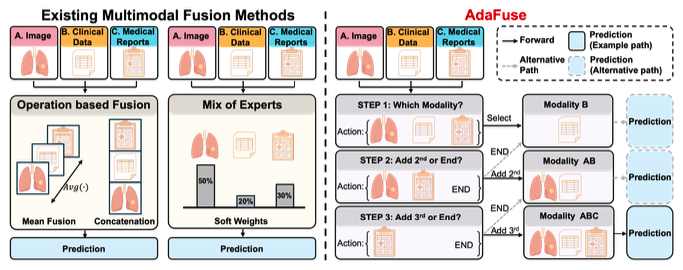
\includegraphics[width=1.04\linewidth,height=0.62\textheight,keepaspectratio]{figures/Adafuse/fig1.png}
\vspace{0.45em}
\large
\begin{minipage}{0.88\textwidth}
\centering
기존 multimodal learning은 주로 주어진 modality들을\\
어떻게 fusion할지에 집중했다.
\end{minipage}
\vspace{0.55em}

{\Large\color{AccentOrange}\bfseries 핵심 질문}\\[0.1em]
{\large\bfseries 예측에 꼭 모든 modality를 써야 할까?}
\end{frame}
% Speaker note:
% 이 슬라이드는 기존 연구가 concat, mean, tensor, MoE처럼 modality를 어떻게 결합할지에 주로 집중했다는 점에서 시작한다.
% AdaFuse의 질문은 fusion rule 자체보다, 특정 환자에게 모든 modality가 정말 필요한가로 이동한다.
% 핵심은 weight를 조정하는 것이 아니라 modality를 아예 사용하지 않는 hard selection이다.

\begin{frame}[t]{Dataset \& Feature Inputs}
\normalsize
\begin{block}{Dataset}
\centering
NLST lung cancer risk prediction \quad|\quad
Train 1,847 / Test 462 \quad|\quad
Positive rate \(\approx 6\%\)
\end{block}
\vspace{0.35em}
\begin{columns}[T,onlytextwidth]
\begin{column}{0.31\textwidth}
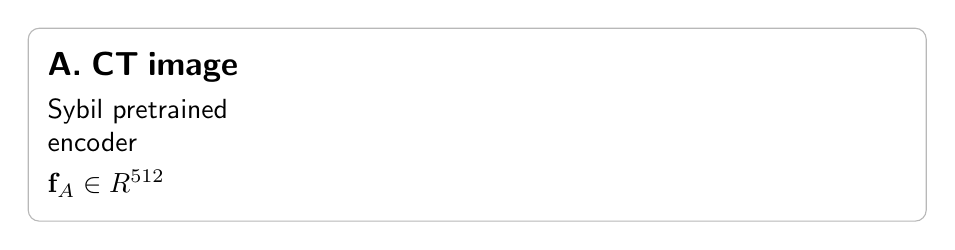
\begin{tikzpicture}
\node[
  draw=LineGray, rounded corners=4pt, fill=white,
  text width=0.90\linewidth, minimum height=2.45cm,
  inner sep=7pt, align=left
] {
{\large\bfseries A. CT image}\\[0.35em]
Sybil pretrained\\
encoder\\[0.3em]
\(\mathbf{f}_A\in\mathbb{R}^{512}\)
};
\end{tikzpicture}
\end{column}
\begin{column}{0.31\textwidth}
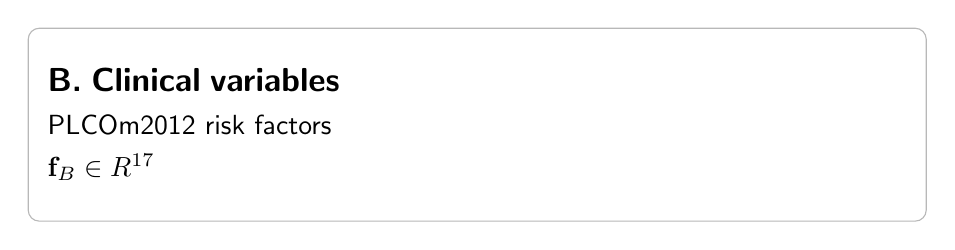
\begin{tikzpicture}
\node[
  draw=LineGray, rounded corners=4pt, fill=white,
  text width=0.90\linewidth, minimum height=2.45cm,
  inner sep=7pt, align=left
] {
{\large\bfseries B. Clinical variables}\\[0.35em]
PLCOm2012 risk factors\\[0.3em]
\(\mathbf{f}_B\in\mathbb{R}^{17}\)
};
\end{tikzpicture}
\end{column}
\begin{column}{0.31\textwidth}
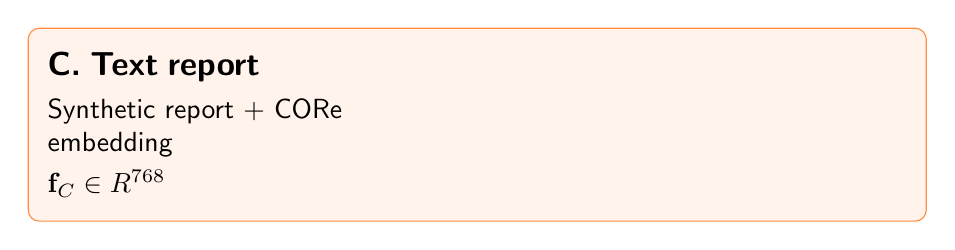
\begin{tikzpicture}
\node[
  draw=AccentOrange, rounded corners=4pt, fill=SoftOrange!45,
  text width=0.90\linewidth, minimum height=2.45cm,
  inner sep=7pt, align=left
] {
{\large\bfseries C. Text report}\\[0.35em]
Synthetic report + CORe\\
embedding\\[0.3em]
\(\mathbf{f}_C\in\mathbb{R}^{768}\)
};
\end{tikzpicture}
\end{column}
\end{columns}
\vspace{0.3em}
\begin{center}
\begin{tikzpicture}[
  font=\small,
  feat/.style={draw=AccentOrange, rounded corners=3pt, fill=SoftOrange!35, minimum width=1.25cm, inner sep=5pt, align=center},
  enc/.style={draw=LineGray, rounded corners=3pt, fill=white, minimum width=2.35cm, inner sep=5pt, align=center},
  emb/.style={draw=AccentOrange, rounded corners=3pt, fill=white, minimum width=1.45cm, inner sep=5pt, align=center},
  note/.style={draw=LineGray, rounded corners=3pt, fill=white, inner sep=5pt, align=center},
  arr/.style={-{Latex[length=2mm]}, draw=AccentOrange, thick}
]
\node[feat] (fa) at (-4.1,0) {\(\mathbf{f}_A\)};
\node[feat] (fb) at (0,0) {\(\mathbf{f}_B\)};
\node[feat] (fc) at (4.1,0) {\(\mathbf{f}_C\)};

\node[enc] (ea) at (-4.1,-0.9) {CT encoder};
\node[enc] (eb) at (0,-0.9) {Clinical encoder};
\node[enc] (ec) at (4.1,-0.9) {Text encoder};

\node[emb] (ha) at (-4.1,-1.8) {\(\mathbf{h}_A\in\mathbb{R}^{32}\)};
\node[emb] (hb) at (0,-1.8) {\(\mathbf{h}_B\in\mathbb{R}^{32}\)};
\node[emb] (hc) at (4.1,-1.8) {\(\mathbf{h}_C\in\mathbb{R}^{32}\)};

\node[note] (shared) at (0,-2.55) {각 modality는 별도 encoder path를 거쳐 공통 32D representation으로 projection};

\draw[arr] (fa) -- (ea);
\draw[arr] (fb) -- (eb);
\draw[arr] (fc) -- (ec);
\draw[arr] (ea) -- (ha);
\draw[arr] (eb) -- (hb);
\draw[arr] (ec) -- (hc);
\end{tikzpicture}
\end{center}
\end{frame}
% Speaker note:
% 이 논문에서 text modality는 실제 판독문이 아니라 structured variable로 생성된 synthetic report이므로,
% 결과 해석 시 주의가 필요하다.

\begin{frame}[t]{Overall AdaFuse Framework}
\centering
\vspace{1.15em}
\vfill
\makebox[\textwidth][c]{%
  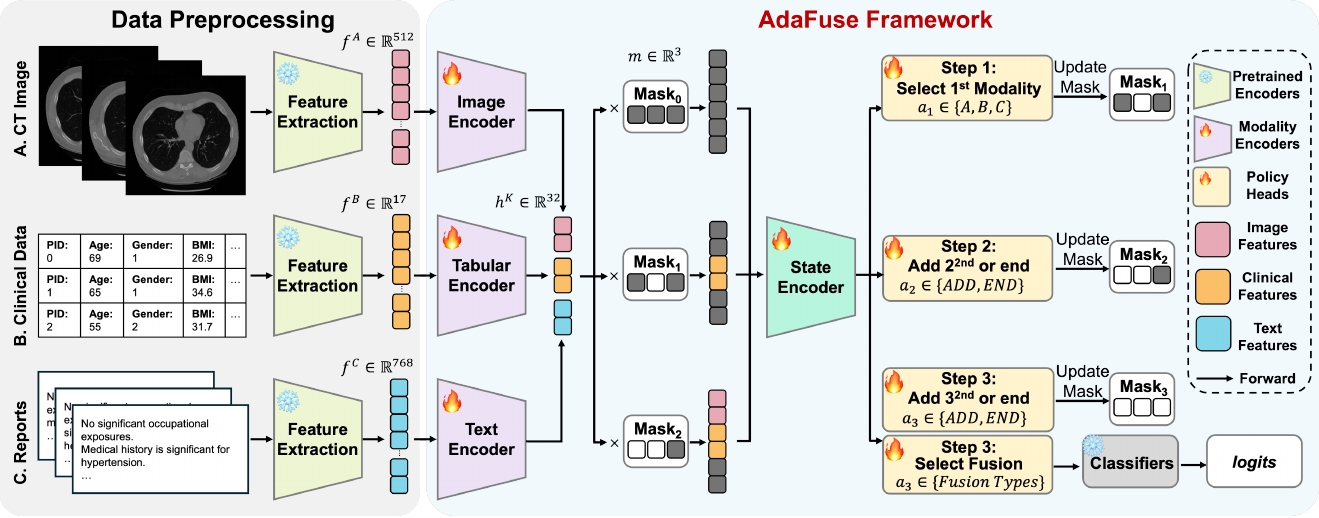
\includegraphics[width=0.96\paperwidth,height=0.78\textheight,keepaspectratio]{figures/Adafuse/fig2.png}%
}
\vfill
\end{frame}
% Speaker note:
% Figure 2가 방법론의 중심 그림이다. 발표에서는 각 모듈을 길게 분해하기보다,
% encoder-state-policy-classifier의 흐름을 먼저 잡아주는 것이 좋다.

\begin{frame}[t]{State Encoder and Policy Head}
\small
\centering
\textbf{Policy network는 현재까지 선택된 modality state를 보고 다음 action의 확률분포를 출력한다.}
\vspace{0.55em}

\begin{columns}[T,onlytextwidth]
\begin{column}{0.49\textwidth}
\begin{block}{1. State Encoder}
\centering
{\large
\[
s_t =
g_\theta([h_A \odot m_A;\, h_B \odot m_B;\, h_C \odot m_C;\, \mathbf{m}])
\]
}
\vspace{-0.8em}
\footnotesize
\begin{itemize}
  \item \(h_A,h_B,h_C\): 32D encoded modality features
  \item \(\mathbf{m}\in\{0,1\}^3\): selected modality mask
  \item unselected modality는 zero-out
  \item output: \(s_t\in\mathbb{R}^{64}\)
\end{itemize}
\vspace{0.15em}
\textcolor{AccentOrange}{\textbf{선택된 modality와 feature 정보를 64D state vector로 요약}}
\end{block}
\end{column}

\begin{column}{0.49\textwidth}
\begin{block}{2. Policy Head}
\centering
{\Large
\[
\pi_\theta(a_t|s_t)=\mathrm{softmax}(l_t/\tau)
\]
}
\vspace{-0.8em}
\footnotesize
\begin{itemize}
  \item 64D state vector \(s_t\)를 입력으로 받음
  \item step-specific head가 action logits \(l_t\) 출력
  \item Training: temperature 기반 sampling
  \item Inference: greedy decoding
\end{itemize}
\vspace{0.15em}
\textcolor{AccentOrange}{\textbf{다음 action에 대한 확률분포 생성}}
\end{block}
\end{column}
\end{columns}

\end{frame}
% Speaker note:
% Policy network는 폐암 확률을 직접 예측하는 것이 아니라, 현재 state에서 어떤 action을 취할지 결정하는 controller이다.
% action에는 modality 선택, 추가/종료, fusion method 선택이 포함된다.
% 최종적으로 선택된 modality-fusion 조합에 해당하는 classifier가 실제 risk prediction을 수행한다.

\begin{frame}[t]{Fusion Methods}
\small
\centering
{\large
\[
h_A,h_B,h_C\in\mathbb{R}^{32}
\]
}
\vspace{-0.65em}
\begin{columns}[T,onlytextwidth]
\begin{column}{0.32\textwidth}
\begin{tikzpicture}
\node[
  draw=LineGray, rounded corners=4pt, fill=white,
  text width=0.96\linewidth, minimum height=3.25cm,
  inner sep=7pt, align=center
] {
{\Large\bfseries\color{AccentOrange} Concat}\\[0.35em]
{\Large \([h_A;h_B;h_C]\)}\\[0.35em]
\footnotesize 선택된 modality feature를\\그대로 concatenate\\[0.45em]
\scriptsize Triple: \(32\times3=96\)D
};
\end{tikzpicture}
\end{column}
\begin{column}{0.32\textwidth}
\begin{tikzpicture}
\node[
  draw=LineGray, rounded corners=4pt, fill=white,
  text width=0.96\linewidth, minimum height=3.25cm,
  inner sep=7pt, align=center
] {
{\Large\bfseries\color{AccentOrange} Mean}\\[0.35em]
{\Large \((h_A+h_B+h_C)/3\)}\\[0.35em]
\footnotesize 공통 32D representation을\\element-wise average\\[0.45em]
\scriptsize Triple output은 32D
};
\end{tikzpicture}
\end{column}
\begin{column}{0.32\textwidth}
\begin{tikzpicture}
\node[
  draw=AccentOrange, rounded corners=4pt, fill=SoftOrange!35,
  text width=0.96\linewidth, minimum height=3.25cm,
  inner sep=7pt, align=center
] {
{\Large\bfseries\color{AccentOrange} Tensor}\\[0.25em]
{\large \([h_A;1]\otimes[h_B;1]\otimes[h_C;1]\)}\\[0.35em]
\footnotesize modality 간 multiplicative\\interaction을 명시적으로 생성\\[0.35em]
\scriptsize Naive 32D 기준:\\
\scriptsize triple \((32+1)^3\)
};
\end{tikzpicture}
\end{column}
\end{columns}
\vspace{0.45em}
\begin{block}{Fusion step}
\centering\small
환자마다 어떤 modality 조합을 쓰느냐에 따라 최적 fusion 방식도 달라질 수 있다는 가정
\end{block}
\end{frame}
% Speaker note:
% 이 슬라이드는 baseline 나열보다 fusion operator 자체를 설명하는 데 집중한다.
% Concat은 차원이 modality 수에 비례해 증가하고, mean은 32D를 유지한다.
% Tensor는 interaction term을 만들지만 차원이 급격히 커지며, 논문 Appendix의 (16+1)^n 표기와 본문의 32D encoder output 설명 사이에 불명확성이 있다.

\begin{frame}[t]{Reward Design}
\small
\begin{center}
{\Large
\[
r = r_{\mathrm{BCE}} + \lambda_{\mathrm{AUC}}\cdot r_{\mathrm{AUC}}
\qquad
r_{\mathrm{BCE}} = y\log\hat p+(1-y)\log(1-\hat p)
\]
}
\end{center}
\vspace{-0.35em}
\begin{columns}[T,onlytextwidth]
\begin{column}{0.50\textwidth}
\begin{block}{BCE reward}
\begin{itemize}
  \item Negative BCE 형태
  \item 개별 환자 예측이 정답에 가까울수록 reward 증가
\end{itemize}
\end{block}
\end{column}
\begin{column}{0.48\textwidth}
\begin{block}{AUC reward}
\begin{itemize}
  \item mini-batch 내 positive/negative 쌍별 비교
  \item 암 환자 score가 정상인 score보다 반드시 높아야 reward를 받음
  \item \(\rightarrow\) 모델이 암 환자를 정상인과 명확히 구분하도록 강제
\end{itemize}
\end{block}
\end{column}
\end{columns}
\vspace{0.45em}
\begin{block}{목적}
\centering\large
좋은 예측과 좋은 ranking을 만든 modality/fusion 선택 경로에 더 높은 reward를 부여
\end{block}
\end{frame}
% Speaker note:
% Reward design은 이번 modality 선택이 좋은 선택이었는지를 평가하는 부분이다.
% BCE reward는 개별 예측 정확도에 가깝고, AUC reward는 mini-batch 안의 positive/negative pairwise ranking을 반영한다.

\begin{frame}[t]{Policy Gradient Optimization}
\small
\vspace{0.05em}
\begin{center}
\large\bfseries
좋은 선택은 강화하고, 탐색은 유지하며, 예측은 안정화한다.
\end{center}
\vspace{-0.2em}
\begin{center}
{\Large
\[
L=L_{\mathrm{PG}}-\lambda_{\mathrm{ent}}\sum_t H(\pi_\theta(\cdot\mid s_t))+\lambda_{\mathrm{sup}}L_{\mathrm{BCE}}
\]
}
\vspace{-0.8em}
{\scriptsize\textcolor{AccentOrange}{%
\(H(\pi_\theta(\cdot\mid s_t))\): entropy
}}
\end{center}
\vspace{-0.45em}
\begin{enumerate}
  \item \textbf{Policy gradient loss}\\[-0.1em]
  \footnotesize Reward가 높은 modality/fusion trajectory의 선택 확률을 높임

  \vspace{0.45em}
  \item \textbf{Entropy regularization}\\[-0.1em]
  \footnotesize Policy가 초기에 한 action으로 collapse되는 것을 방지

  \vspace{0.45em}
  \item \textbf{Supervised BCE loss}\\[-0.1em]
  \footnotesize 예측 결과가 정답 label에 가까워지도록 안정화
\end{enumerate}
\vspace{0.35em}
\begin{block}{Policy gradient term}
\centering
\vspace{-0.2em}
\resizebox{0.98\linewidth}{!}{%
\(\displaystyle
\tau_{\mathrm{traj}}=(a_1,a_2,\ldots)
\quad\Rightarrow\quad
\log\pi_\theta(\tau_{\mathrm{traj}})
=\sum_t\log\pi_\theta(a_t\mid s_t)
\quad\Rightarrow\quad
L_{\mathrm{PG}}
=-\log\pi_\theta(\tau_{\mathrm{traj}})(r-\bar r)
\)
}
\vspace{-0.6em}
\begin{flushright}
\scriptsize \(\bar r\): mini-batch 평균 reward\hspace{1.2em}
\end{flushright}
\end{block}
\end{frame}
% Speaker note:
% 이 슬라이드에서는 policy gradient 세부 derivation보다 full objective의 세 항이 각각 무슨 역할을 하는지 설명하면 된다.
% L_PG는 reward가 좋은 trajectory의 확률을 올리는 항이고, entropy는 exploration collapse를 막으며, supervised BCE는 classifier prediction에 안정적인 gradient를 제공한다.

\begin{frame}[t]{Main Results}
\begin{columns}[T,onlytextwidth]
\begin{column}{0.68\textwidth}
\centering
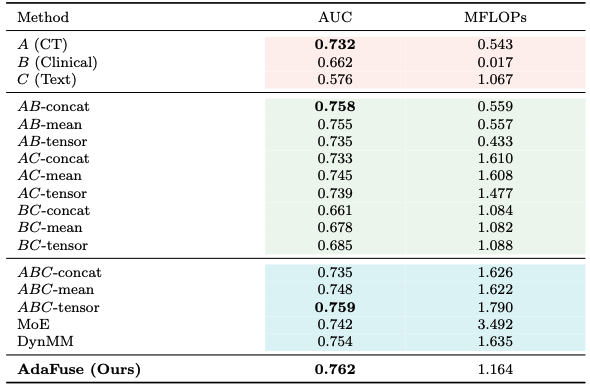
\includegraphics[width=\linewidth,height=0.70\textheight,keepaspectratio]{figures/Adafuse/table1.png}
\vspace{-0.15em}
\begin{block}{MFLOPs}
\scriptsize
모델이 한 번 예측할 때 필요한 부동소수점 연산 수를 백만 단위로 나타낸 계산 비용 지표
\end{block}
\end{column}
\begin{column}{0.30\textwidth}
\small
\begin{block}{Key observations}
\footnotesize
\textbf{1. Best AUC, 하지만 margin은 작음}\\
AdaFuse 0.762 vs ABC-tensor 0.759

\vspace{0.75em}
\textbf{2. More modalities \(\neq\) better performance}\\
AB-concat 0.758 \(>\) ABC-concat 0.735

\vspace{0.75em}
\textbf{3. 더 나은 AUC--cost trade-off}\\
AdaFuse 1.164 MFLOPs\\
DynMM 1.635, MoE 3.492
\end{block}
\end{column}
\end{columns}
\end{frame}
% Speaker note:
% 결과를 과장하지 않는 것이 중요하다. AdaFuse가 가장 높지만 ABC-tensor와 차이는 매우 작다.
% 동시에 AB-concat이 ABC-concat보다 좋은 점은 modality를 더 추가한다고 항상 성능이 좋아지지는 않는다는 점을 보여준다.
% FLOPs 관점에서는 AdaFuse가 DynMM이나 MoE보다 낮은 비용으로 경쟁력 있는 AUC를 보인다.

\begin{frame}[t]{Training Configuration Ablation}
\small
\centering
\vspace{0.45em}
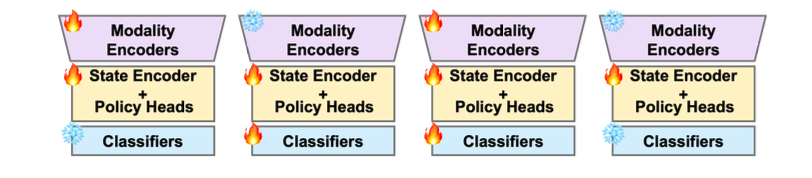
\includegraphics[width=0.98\linewidth,height=0.41\textheight,keepaspectratio]{figures/Adafuse/fig4.png}
\vspace{0.15em}
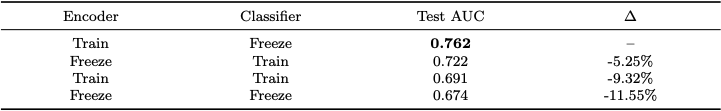
\includegraphics[width=0.88\linewidth,height=0.22\textheight,keepaspectratio]{figures/Adafuse/table2.png}
\vspace{0.2em}
\begin{minipage}{0.86\textwidth}
\begin{block}{핵심 해석}
\footnotesize
\textbf{1. Classifier는 freeze하는 것이 가장 좋음}\\
Train encoder + Freeze classifier = 0.762

\vspace{0.45em}
\textbf{2. Classifier까지 학습하면 reward signal이 불안정해질 수 있음}\\
선택된 classifier만 gradient를 자주 받아, 덜 선택된 classifier는 undertrained될 수 있음.
\end{block}
\end{minipage}
\end{frame}
% Speaker note:
% 이 ablation은 AdaFuse training에서 classifier를 고정하는 것이 단순한 구현 선택이 아니라 핵심 안정화 장치임을 보여준다.
% classifier까지 train하면 선택 빈도에 따라 classifier 학습량이 달라져 reward signal이 흔들릴 수 있다.

\begin{frame}[t]{Learning Objective Ablation}
\centering
\vspace{0.55em}
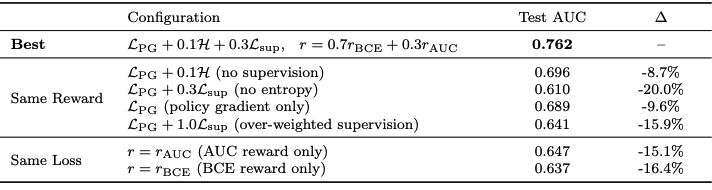
\includegraphics[width=0.96\linewidth,height=0.45\textheight,keepaspectratio]{figures/Adafuse/table3.png}
\vspace{0.35em}
\begin{columns}[T,onlytextwidth]
\begin{column}{0.49\textwidth}
\begin{block}{1. Same Reward}
\scriptsize
\begin{itemize}
  \item Entropy 제거가 가장 치명적\\
  \(\rightarrow\) 15개 조합 탐색에서 초기 다양성이 결정적
  \item Supervision이 너무 강하면 selection 학습이 약해짐\\
  \(\rightarrow\) reward signal을 압도하면 policy가 selection 자체를 못 배움
\end{itemize}
\end{block}
\end{column}
\begin{column}{0.49\textwidth}
\begin{block}{2. Same Loss}
\scriptsize
\begin{itemize}
  \item BCE/AUC 단독 reward는 모두 성능 하락
  \item positive rate 6\% 환경에서\\
  BCE만으로는 ranking signal이 부족하고,\\
  AUC만으로는 gradient가 sparse함\\
  \(\rightarrow\) 두 reward가 상호보완적
\end{itemize}
\end{block}
\end{column}
\end{columns}
\end{frame}
% Speaker note:
% Objective ablation에서는 entropy와 supervised term이 매우 중요하게 나온다.
% 특히 no entropy의 성능 저하는 policy가 너무 빨리 좁은 선택으로 collapse될 수 있음을 시사한다.

\setbeamertemplate{footline}{%
  \nointerlineskip%
  \color{LineGray}\rule{\paperwidth}{0.035cm}%
  \vskip0.04cm%
  \makebox[\paperwidth]{%
    \hspace{0.75cm}\scriptsize\color{AccentOrange}LDTL \hspace{0.6em}|\hspace{0.6em} Sequential Clinical Diagnosis%
    \hfill\scriptsize\color{AccentOrange}\insertframenumber\,/\,\inserttotalframenumber\hspace{0.75cm}%
  }%
  \vskip0.08cm%
}

\section{LDTL}

\begin{frame}[t]
\vspace{2.1em}
\begin{center}
{\Large\bfseries Uncertainty-Guided Latent Diagnostic Trajectory Learning for Sequential Clinical Diagnosis}\\[0.7em]
{\normalsize\color{AccentOrange}Sequential evidence acquisition for clinical diagnosis}\\[1.0em]
{\small Xuyang Shen, Haoran Liu, Dongjin Song, Martin Renqiang Min}\\[0.25em]
{\small arXiv 2026}
\end{center}
\end{frame}
% Speaker note:
% LDTL은 diagnosis를 full-information prediction으로 두지 않고, evidence를 순차적으로 획득하면서 언제 멈출지 결정하는 문제로 본다.
% 발표에서는 방법 자체보다 trajectory-level claim과 실제 구현 사이의 간극을 비판적으로 보는 흐름이 중요하다.

\begin{frame}[t]{Problem: 기존 LLM Diagnosis의 한계}
\small
\begin{columns}[T,onlytextwidth]
\begin{column}{0.32\textwidth}
\begin{block}{1. Full-information assumption}
\footnotesize
모든 정보를 미리 준다고 가정.\\[0.35em]
\textbf{\(\rightarrow\)} 실제 임상과 괴리
\end{block}
\end{column}
\begin{column}{0.32\textwidth}
\begin{block}{2. No path supervision}
\footnotesize
Sequential하게 다루더라도 어떤 검사 순서가 좋은지 label이 없음.\\[0.35em]
\textbf{\(\rightarrow\)} good path를 supervised 학습할 수 없음
\end{block}
\end{column}
\begin{column}{0.32\textwidth}
\begin{block}{3. Reward-only optimization}
\footnotesize
Terminal reward만으로는 중간 경로의 질을 직접 평가하기 어려움.\\[0.35em]
\textbf{\(\rightarrow\)} path 구조 제어와 학습 안정성이 약함
\end{block}
\end{column}
\end{columns}
\vspace{0.75em}
\begin{block}{핵심 질문}
\centering\small\bfseries
정답 경로 label 없이 어떻게 좋은 diagnostic trajectory를 정의하고 학습할 것인가?
\end{block}
\end{frame}
% Speaker note:
% 이 논문은 정답 disease label은 있지만 어떤 검사를 어떤 순서로 선택해야 좋은지에 대한 label이 없는 상황을 다룬다.
% 핵심은 full-information prediction의 한계를 넘어서, 경로 label 없이 좋은 trajectory를 간접적으로 정의해야 한다는 점이다.
% 그래서 LDTL은 diagnostic improvement를 이용해 IG 기반 posterior target을 만든다.

\begin{frame}[t]{Overall Framework: Planning Agent + Diagnostic Agent}
\centering

\includegraphics[width=0.98\linewidth,height=0.58\textheight,keepaspectratio]{figures/LDTL/fig2.png}
\vspace{0.2em}
\begin{columns}[T,onlytextwidth]
\begin{column}{0.49\textwidth}
\begin{block}{Planning LLM agent}
\footnotesize 현재 상태 \(h_t\)에서 다음 검사 action \(a_t\)를 선택한다.
\end{block}
\end{column}
\begin{column}{0.49\textwidth}
\begin{block}{Diagnostic LLM agent}
\footnotesize 업데이트된 상태 \(h_{t+1}\)에서 disease prediction, confidence, stop 여부를 낸다.
\end{block}
\end{column}
\end{columns}
\vspace{0.15em}
\centering\footnotesize \(h_t \rightarrow a_t \rightarrow h_{t+1} \rightarrow \hat y,\ \mathrm{confidence},\ \mathrm{stop}\)
\end{frame}
% Speaker note:
% Figure 2는 LDTL 전체 구조다. Planning agent가 검사 category를 고르고, Diagnostic agent가 새 evidence를 반영해 진단과 confidence를 업데이트한다.
% 아래쪽 training block은 posterior action distribution을 구성해 planner policy를 맞추는 부분이다.

\begin{frame}[t]{Problem Formulation}
\small
\begin{columns}[T,onlytextwidth]
\begin{column}{0.52\textwidth}
\begin{block}{Notation}
\begin{itemize}
  \item 초기 상태: \(h_0\)
  \item Action: \(a_t \in \mathcal{A}\)
  \item Action space: \(\{\mathrm{lab},\mathrm{physical},\mathrm{image}\}\)
  \item 상태 업데이트: \(h_{t+1}=\mathrm{Update}(h_t,a_t)\)
\end{itemize}
\end{block}
\end{column}
\begin{column}{0.45\textwidth}
\begin{block}{Trajectory}
\[
z=(a_1,\dots,a_T)
\]
\footnotesize \(z\)는 미리 주어진 label이 아니라 step-by-step 선택이 누적되어 만들어지는 검사 경로다.
\end{block}
\end{column}
\end{columns}
\vspace{0.5em}
\begin{block}{핵심 메시지}
\centering\Large\bfseries
목표는 accurate diagnosis와 fewer tests 사이의 균형
\end{block}
\end{frame}
% Speaker note:
% 여기서 action은 individual laboratory item이 아니라 lab, physical, image 같은 category-level action이다.
% trajectory z는 planner가 각 step에서 선택한 action sequence이며, 데이터셋에 정답 trajectory label로 들어 있는 것은 아니다.

\begin{frame}[t]{Why ``Latent'' Trajectory?}
\small
\begin{columns}[T,onlytextwidth]
\begin{column}{0.47\textwidth}
\begin{block}{데이터에서 관측되는 것}
\begin{itemize}
  \item 초기 patient state \(h_0\)
  \item 사용 가능한 test results: lab / physical / image
  \item 최종 disease label \(y\)
\end{itemize}
\end{block}
\end{column}
\begin{column}{0.47\textwidth}
\begin{alertblock}{데이터에서 관측되지 않는 것}
\begin{itemize}
  \item Optimal diagnostic trajectory \(z^*\)
  \item 어떤 test를 먼저 획득해야 하는가?
  \item 언제 diagnosis를 종료해야 하는가?
\end{itemize}
\end{alertblock}
\end{column}
\end{columns}
\vspace{1.0em}
\begin{block}{핵심 메시지}
\centering
``Latent''는 patient information이 숨겨져 있다는 뜻이 아니다.\\
\vspace{0.2em}
좋은 diagnostic path에 대한 label이 관측되지 않는다는 뜻이다.
\end{block}
\end{frame}
% Speaker note:
% 데이터에는 최종 진단명은 있지만, 어떤 검사를 어떤 순서로 선택해야 좋은지에 대한 정답 trajectory label은 없다.
% 그래서 LDTL은 diagnostic improvement signal을 이용해 좋은 path를 간접적으로 정의한다.

\begin{frame}[t]{What Makes a Good Diagnostic Path?}
\small
\begin{block}{동기}
\footnotesize
\begin{itemize}
  \item 문제: 정답 label \(y\)는 있지만 optimal trajectory \(z^*\)는 없다.
  \item 목표: ``정답 진단에 더 기여하는 경로''를 높은 preference로 표현한다.
\end{itemize}
\end{block}
\vspace{0.45em}
\begin{columns}[T,onlytextwidth]
\begin{column}{0.50\textwidth}
\begin{alertblock}{Trajectory-level}
\centering
\[
q(z\mid h_0,y)=
\frac{\exp(\beta S(z))}
{\sum_{z'\in Z(h_0)}\exp(\beta S(z'))}
\]
\end{alertblock}
\footnotesize
\begin{itemize}
  \item \(S(z)\): trajectory \(z\)가 정답 \(y\)를 얼마나 잘 지지하는가
  \item \(\beta\): 분포의 sharpness 조절
\end{itemize}
\end{column}
\begin{column}{0.47\textwidth}
\begin{block}{Action-level}
\centering
\[
q(a_t\mid h_t,y)=
\sum_{z:\,z_t=a_t}q(z\mid h_0,y)
\]
\end{block}
\footnotesize
Full \(q(z\mid h_0,y)\)가 있다면, \(t\)번째 action이 \(a_t\)인 trajectory posterior를 합산해 action-level teacher를 만들 수 있다.
\end{column}
\end{columns}
\vspace{0.55em}
\begin{alertblock}{한계}
\footnotesize
Trajectory space가 지수적으로 커지므로 모든 \(z\)에 대해 \(S(z)\)를 평가하고
\(q(z\mid h_0,y)\)를 직접 계산하기 어렵다.
\end{alertblock}
\end{frame}
% Speaker note:
% 정답 label y는 있지만 어떤 검사 순서가 좋은지는 데이터에 없다.
% 이 슬라이드는 trajectory-level teacher posterior와 여기서 action-level teacher를 얻는 ideal marginalization을 보여준다.
% 핵심 한계는 trajectory space가 커지면 모든 path의 S(z)를 계산할 수 없다는 점이다.

\begin{frame}[t]{IG Approximation}
\footnotesize
\begin{columns}[T,onlytextwidth]
\begin{column}{0.53\textwidth}
\textcolor{AccentOrange}{\bfseries 근사 아이디어}\quad
\scriptsize 전체 경로 대신 ``이 action 하나를 추가하면 정답 확률이 얼마나 오르는가?''로 대체
\vspace{0.15em}
\centering
\large
\[
\mathrm{IG}(h_t,a)=
\log p_\psi(y\mid h_{t+1})
-\log p_\psi(y\mid h_t)
\]
\vspace{-0.4em}
\[
q(a\mid h_t,y)\propto
\exp(\mathrm{IG}(h_t,a)/\tau)
\]
\end{column}
\begin{column}{0.44\textwidth}
\begin{block}{Action posterior}
\centering
\large
\[
q(a\mid h_t,y)
\]
\vspace{-0.3em}
\footnotesize
현재 state에서 각 candidate action의 IG를 계산해 teacher action distribution으로 변환한다.
\end{block}
\end{column}
\end{columns}
\vspace{-0.05em}
\keymessage{trajectory-level posterior를 one-step information gain으로 근사한다.}
\end{frame}
% Speaker note:
% 이상적으로는 trajectory posterior를 action posterior로 marginalize하고 싶지만, 가능한 path가 너무 많아 직접 계산이 어렵다.
% 그래서 LDTL은 action 하나를 추가했을 때 정답 y의 probability가 얼마나 증가하는지, 즉 one-step information gain으로 q(a|h_t,y)를 근사한다.

\begin{frame}[t]{Train the Planner to Follow the Teacher}
\small
\begin{block}{동기}
\begin{itemize}
  \item 목표: planner \(\pi_\theta\)가 teacher \(q\)를 모방하도록 학습
\end{itemize}
\end{block}
\vspace{0.2em}
\begin{alertblock}{Planner loss}
\centering
\large
\[
L_{\mathrm{planner}}=
\sum_{t=1}^{T}
\mathrm{KL}\!\left(
q(a\mid h_t,y)\,\|\,\pi_\theta(a\mid h_t)
\right)
\]
\end{alertblock}
\vspace{0.25em}
\begin{block}{학습 방향}
\footnotesize
teacher distribution \(q(a\mid h_t,y)\)와 planner policy \(\pi_\theta(a\mid h_t)\) 사이의 차이를 줄인다.
\end{block}
\end{frame}
% Speaker note:
% planner는 reward trial-and-error로 직접 학습하기보다, diagnostic agent와 정답 label로 만든 teacher distribution q를 따라가도록 KL로 학습된다.
% 그래서 발표에서는 LDTL을 standard RL이라기보다 information gain 기반 soft-label imitation learning에 가깝다고 설명하면 된다.

\begin{frame}[t]{Dataset and Action Space}
\small
\begin{columns}[T,onlytextwidth]
\begin{column}{0.52\textwidth}
\begin{block}{MIMIC-CDM}
\begin{itemize}
  \item 2,400 inpatient cases
  \item 4 abdominal diseases:
  \begin{itemize}
    \item appendicitis (충수염)
    \item cholecystitis (담낭염)
    \item diverticulitis (게실염)
    \item pancreatitis (췌장염)
  \end{itemize}
  \item Split: 70 / 10 / 20
  \item Backbone: Llama-3-8B + LoRA
\end{itemize}
\end{block}
\end{column}
\begin{column}{0.45\textwidth}
\begin{block}{Action space}
\begin{itemize}
  \item lab
  \item physical
  \item image
\end{itemize}
\end{block}
\end{column}
\end{columns}
\end{frame}
% Speaker note:
% MIMIC-CDM은 복부 질환 네 가지를 다루며, action space는 physical examination, imaging studies, laboratory tests 세 category다.
% 이 abstraction은 실제 임상 test acquisition보다 훨씬 coarse할 수 있다는 점을 염두에 두어야 한다.

\begin{frame}[t]{Main Results}
\centering

\includegraphics[width=0.98\linewidth,height=0.42\textheight,keepaspectratio]{figures/LDTL/table1.png}
\vspace{0.15em}
\begin{columns}[T,onlytextwidth]
\begin{column}{0.43\textwidth}
\begin{block}{결과 구조}
\scriptsize
\textbf{Upper bound}\\
SFT-all 94.2 \(\rightarrow\) 모든 정보를 다 봤을 때 성능

\vspace{0.45em}
\textbf{Sequential baselines}\\
Random 84.8, ReAct 74.9, LA-CDM 81.3

\vspace{0.45em}
\textbf{LDTL}\\
93.4 \(\rightarrow\) SFT-all에 근접, sequential 중 최고
\end{block}
\end{column}
\begin{column}{0.55\textwidth}
\begin{block}{의미}
\scriptsize
\textbf{긍정적 해석}\\
Sequential baselines 중 최고 성능이며, SFT-all과 0.8\% 차이
\(\rightarrow\) sequential 제약 하에서 거의 upper bound에 도달

\vspace{0.45em}
\textbf{비판적 시각}\\
Random planner 84.8이 ReAct보다 높음
\(\rightarrow\) action space가 3개뿐이라 random도 잘 됨
\(\rightarrow\) LDTL 개선이 framework 때문인지 task 난이도 때문인지 불분명

\vspace{0.45em}
\textbf{클래스별 패턴}\\
Diverticulitis는 LDTL이 random보다 낮음
\(\rightarrow\) 일부 class에서는 trajectory learning이 오히려 해가 될 수 있음
\end{block}
\end{column}
\end{columns}
\end{frame}
% Speaker note:
% LDTL은 sequential setting에서 가장 좋은 결과를 보이고, complete information으로 fine-tune한 SFT-all에 가깝다.
% 그러나 random planner가 84.8로 높다는 점은 lab/physical/image category 중 하나만 열어도 강한 단서가 생기는 task일 수 있음을 시사한다.

\begin{frame}[t]{Case Study: Effect of Latent Path Regularization}
\centering

\includegraphics[width=0.98\linewidth,height=0.52\textheight,keepaspectratio]{figures/LDTL/fig3.png}
\vspace{0.25em}
\begin{columns}[T,onlytextwidth]
\begin{column}{0.49\textwidth}
\small
\begin{itemize}
  \item Patient 1: LDTL은 더 짧은 경로로 correct diagnosis에 도달한다.
  \item w/o LP는 추가 imaging 후 lab test까지 요청한다.
\end{itemize}
\end{column}
\begin{column}{0.49\textwidth}
\begin{block}{Interpretation}
\footnotesize Figure 3는 latent path regularization이 informative action을 더 일찍 선택하도록 돕는다는 정성적 예시다.
\end{block}
\end{column}
\end{columns}
\end{frame}
% Speaker note:
% Figure 3는 정량 결과가 아니라 case study다.
% LDTL과 w/o LP의 diagnostic path를 비교해, posterior-guided training이 불필요한 검사나 premature termination을 줄인다는 논문의 주장을 시각적으로 보여준다.

\begin{frame}[t]{Ablation + Efficiency}
\begin{columns}[T,onlytextwidth]
\begin{column}{0.47\textwidth}
\centering

\includegraphics[width=\linewidth,height=0.30\textheight,keepaspectratio]{figures/LDTL/table2.png}
\vspace{0.25em}

\includegraphics[width=\linewidth,height=0.39\textheight,keepaspectratio]{figures/LDTL/fig4.png}
\end{column}
\begin{column}{0.50\textwidth}
\small
\begin{block}{Ablation}
\begin{itemize}
  \item Random selection: 84.8
  \item w/o LP: 88.6
  \item LDTL: 93.4
\end{itemize}
\end{block}
\begin{itemize}
  \item State-conditioned planner만으로도 random보다 좋아진다.
  \item Trajectory-level posterior alignment가 추가 향상을 만든다고 주장한다.
  \item LDTL은 one-step termination이 많고 three-step trajectory가 적다.
\end{itemize}
\begin{alertblock}{Discussion / Concern}
\footnotesize Termination이 정말 calibrated confidence로 잘 결정되는지, confidence 학습 방식은 명확하지 않다.
\end{alertblock}
\end{column}
\end{columns}
\end{frame}
% Speaker note:
% Table 2는 latent path regularization의 효과를 보여준다. w/o LP도 random보다 좋지만, LDTL이 추가로 상승한다.
% Figure 4는 LDTL이 더 빨리 멈춘다는 evidence로 제시되지만, confidence calibration 자체가 어떻게 보장되는지는 다소 불명확하다.

\begin{frame}[t]{Three Acquisition Objectives with Alternative Branches}
\centering
\vspace{0.05em}
\resizebox{0.96\linewidth}{0.75\textheight}{%
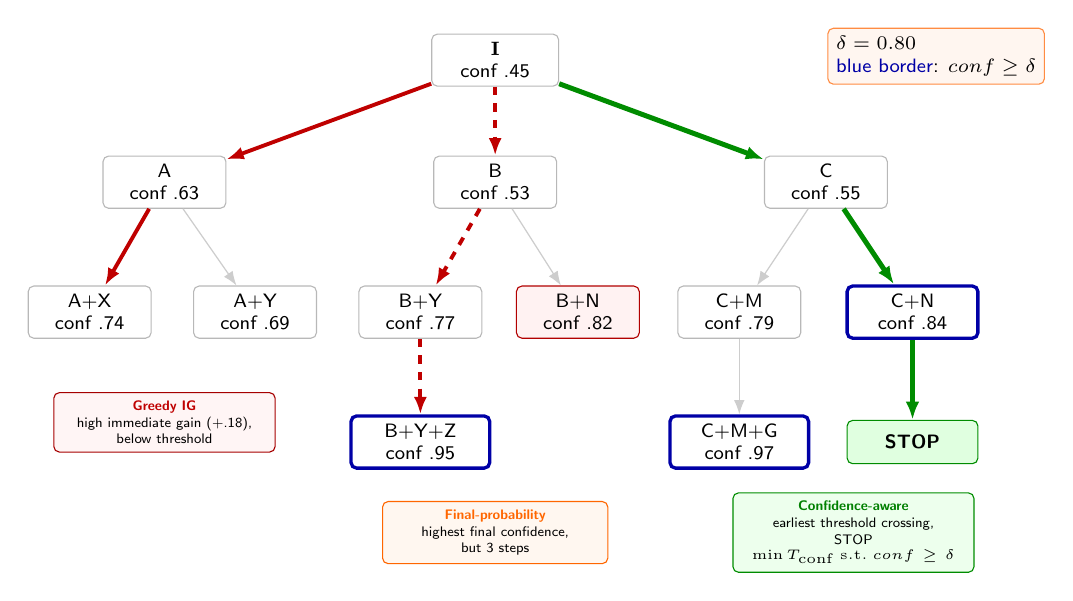
\begin{tikzpicture}[x=1cm,y=1cm]
  \node[lowConfNode, text width=1.4cm, minimum height=0.62cm] (O) at (0,0)
    {\(\mathbf{I}\)\\conf .45};

  \node[lowConfNode, text width=1.35cm] (A) at (-4.2,-1.55) {A\\conf .63};
  \node[lowConfNode, text width=1.35cm] (B) at (0,-1.55) {B\\conf .53};
  \node[lowConfNode, text width=1.35cm] (C) at (4.2,-1.55) {C\\conf .55};

  \node[lowConfNode, text width=1.35cm] (AX) at (-5.15,-3.2) {A+X\\conf .74};
  \node[lowConfNode, text width=1.35cm] (AY) at (-3.05,-3.2) {A+Y\\conf .69};

  \node[lowConfNode, text width=1.35cm] (BY) at (-0.95,-3.2) {B+Y\\conf .77};
  \node[lowConfNode, draw=red!70!black, fill=red!5, text width=1.35cm] (BN) at (1.05,-3.2) {B+N\\conf .82};
  \node[highConfNode, text width=1.55cm] (BYZ) at (-0.95,-4.85) {B+Y+Z\\conf .95};

  \node[lowConfNode, text width=1.35cm] (CM) at (3.1,-3.2) {C+M\\conf .79};
  \node[highConfNode, text width=1.45cm] (CN) at (5.3,-3.2) {C+N\\conf .84};
  \node[highConfNode, text width=1.55cm] (CMG) at (3.1,-4.85) {C+M+G\\conf .97};
  \node[stopNode, text width=1.45cm] (STOP) at (5.3,-4.85) {STOP};

  \draw[greedyEdge] (O) -- (A);
  \draw[finalEdge] (O) -- (B);
  \draw[oursEdge] (O) -- (C);

  \draw[greedyEdge] (A) -- (AX);
  \draw[candidateEdge] (A) -- (AY);

  \draw[finalEdge] (B) -- (BY);
  \draw[finalEdge] (BY) -- (BYZ);
  \draw[candidateEdge] (B) -- (BN);

  \draw[candidateEdge] (C) -- (CM);
  \draw[candidateEdge] (CM) -- (CMG);
  \draw[oursEdge] (C) -- (CN);
  \draw[oursEdge] (CN) -- (STOP);

  \node[draw=red!65!black, fill=red!4, rounded corners=2pt, align=center, text width=2.6cm, font=\tiny, inner sep=3pt] at (-4.2,-4.6)
    {\textbf{\textcolor{red!75!black}{Greedy IG}}\\
     high immediate gain (+.18),\\below threshold};

  \node[draw=orange!80!red, fill=orange!6, rounded corners=2pt, align=center, text width=2.65cm, font=\tiny, inner sep=3pt] at (0,-6.0)
    {\textbf{\textcolor{orange!80!red}{Final-probability}}\\
     highest final confidence,\\but 3 steps};

  \node[draw=green!55!black, fill=green!7, rounded corners=2pt, align=center, text width=2.85cm, font=\tiny, inner sep=3pt] at (4.55,-6.0)
    {\textbf{\textcolor{green!50!black}{Confidence-aware}}\\
     earliest threshold crossing,\\STOP\\[-0.1em]
     \(\min T_{\mathrm{conf}}\ \mathrm{s.t.}\ conf\geq\delta\)};

  \node[draw=AccentOrange, rounded corners=2pt, fill=SoftOrange!35, align=left, inner sep=3pt, font=\scriptsize] at (5.6,0.05)
    {\(\delta=0.80\)\\
     \textcolor{blue!65!black}{blue border}: \(conf\geq\delta\)};
\end{tikzpicture}
}
\vspace{0.06em}

{\tiny
\tikz{\draw[candidateEdge] (0,0)--(0.45,0);} alternative candidate path \quad
\tikz{\draw[greedyEdge] (0,0)--(0.45,0);} Greedy IG selection \quad
\tikz{\draw[finalEdge] (0,0)--(0.45,0);} Final-probability selection \quad
\tikz{\draw[oursEdge] (0,0)--(0.45,0);} confidence-aware selection \quad
\tikz{\node[highConfNode, minimum width=0.34cm, minimum height=0.16cm] at (0,0) {}; } conf \(\geq\delta\) \quad
\tikz{\node[lowConfNode, minimum width=0.34cm, minimum height=0.16cm] at (0,0) {}; } below threshold
}\\[-0.1em]

{\tiny\itshape Goal: reach a reliable diagnosis with minimal evidence.}
\end{frame}
% Speaker note:
% 이 슬라이드는 같은 initial state에서 세 acquisition objective가 서로 다른 경로를 선택하는 conceptual comparison이다.
% Greedy IG는 A의 immediate gain을 보고 들어가지만 threshold를 넘지 못한다.
% Final-probability는 최종 confidence가 높은 긴 trajectory를 선호하지만, B+N처럼 더 이른 confident state를 놓친다.
% Confidence-aware objective는 가장 높은 final confidence가 아니라 가장 이른 reliable diagnosis state에서 멈추는 관점이다.

\end{document}
